\section{Speech in communication}
\label{speech_in_comm}

This section will analyse speech intelligibility with respect to communication. Speech intelligibility is a wide topic which depends on the speech quality, noise and the frequency range. This section will focus on the speech intelligibility frequency range, which might differ from the speech power frequency range, in order to determine the necessary frequency range in electronic systems for communications. First, the speech generation process will be described, as well as speech perception, in order to continue analysing the speech power frequency range and its relation to intelligibility. This will help assess the transducer type that will better fit for the purpose of the study.

\subsection{Speech generation}

One on the most important acoustics factors in human speech is the glottal organ, which makes the fundamental frequency of the voice, $f_0$. The fundamental frequency is not the same for every person, so we will refer to its mean from this point onwards. However, this mean differs between male and female subjects, as well as between different types of communication e.g. talking, yelling or singing. For males, the mean fundamental frequency for conversational speech is \SI{120}{\hertz}, whereas for females it is \SI{200}{\hertz}. The fact that the fundamental frequency is in the low frequency region does not mean that the transmitted sound has only low frequency components. The pathway followed by sound from the glottal organ to the mouth can be represented with a unique transfer function, which heavily impacts on the frequency response \citep{pulkki2015}, and which can vary between subjects. The following \autoref{fig:speech_system} shows the pathway for the soudwaves to propagate from the glottal to the lips.

 \begin{figure}[H]
	\centering
		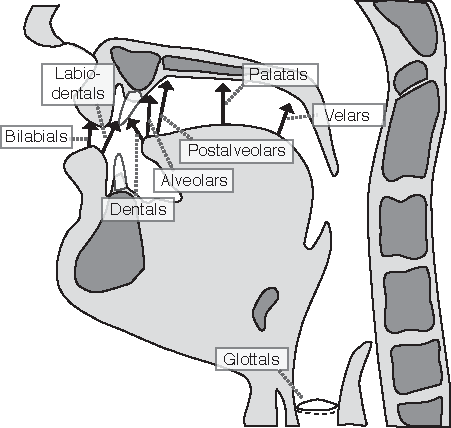
\includegraphics[width=1\textwidth]{glottal}
		\caption{Speech generation pathway from glottals to lips \citep{pulkki2015}}
		\label{fig:speech_system}
\end{figure}

\subsection{Speech frequency range}

As stated before, the transfer function for this system is individual dependent, or more specifically, throat, mouth and nose dependent. The mean length for the throat from the glottal organ to the lips is \SI{17}{\centi\meter} for males and \SI{14}{\centi\meter} for females. While generating speech, glottal oscillations are mixed with "silent" airflow in the throat, which makes turbulences in the transfer of the speech soundwave. This can generate noises and explosive transient-like sounds in the speech output. Another factor to take into account is the position of the lips, which act like a radiation filter, e.g. when pronouncing ''O'' the lips have to be shaped in a specific way, otherwise the generated sound won't be correct. The nose's status also affects the generated sound. For example, generated voice changes if the nose is blocked compared to opened. All these factors for the speech make the frequency range of speech to start below \SI{100}{\hertz} and go upon several \si{\kilo\hertz} \citep{pulkki2015}. The following \autoref{fig:speech_transfer_system} shows a signal block diagram for the speech transfer function.

 \begin{figure}[H]
	\centering
		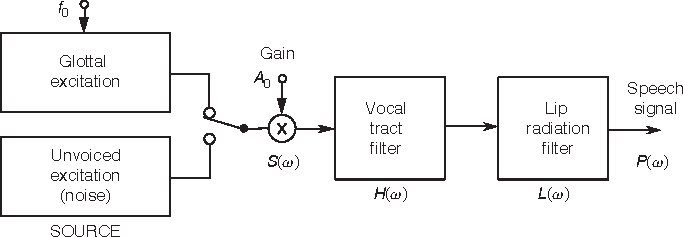
\includegraphics[width=1\textwidth]{speech_transfer}
		\caption{The figure shows a block diagram for the speech transfer function \citep{pulkki2015}}
		\label{fig:speech_transfer_system}
\end{figure}

\subsection{Intelligibility and Speech Power}

In language depending speech, there are some low frequency components generated by the tongue that can go down to \SI{20}{\hertz}. The tongue generates the low frequency components by trilling e.g. ''r'' in Spanish. The highest frequency components are usually generated while singing, and can go up to \SI{7}{\kilo\hertz} \citep{pulkki2015}. At this point, all frequencies above \SI{7}{\kilo\hertz} can be taken as harmonic distortions of the voice. The dynamic range from \SI{20}{\hertz} to \SI{7}{\kilo\hertz} is then the outer limit for speech frequency, but when assessing intelligibility, it might not be affected by the whole range and just a specific area within it.

Speech intelligibility is a measure of how much of a message has been extracted from the recognized phonemes, which are the smallest unit of speech \citep{arl_us_army}. This measure indicates how good words and sentences can be understood in a listening event. Speech intelligibility  is expressed in percentage, indicating the amount of understood speech out of the total received amount. The power spectrum of speech, which was previously analysed and falls within the \SI{20}{\hertz} to \SI{7}{\kilo\hertz} range, is not correlated to the speech intelligibility. This means that the understanding of speech does not have a direct relation with the area of highest speech power. 

Most of the speech power is distributed near the fundamental frequency of the voice, but for speech intelligibility measurements, it was tested that taking out this area would only affect intelligibility by lowering it by a factor below \SI{5}{\percent}. Therefore, when listening to speech, the frequency of the voice might not be observed as its fundamental frequency, but much higher. In fact, \SI{60}{\percent} of the speech intelligibility lays in only \SI{5}{\percent} of the speech power spectrum \citep{arl_us_army}. The spectral centroid of the speech intelligibility frequency varies between different languages, but the deviation is not large. For the English language, the centroid is found at \SI{1.5}{\kilo\hertz} \citep{arl_us_army}. The following \autoref{fig:speech_intelligibility} shows the power and intelligibility in octaves. 

 \begin{figure}[H]
	\centering
		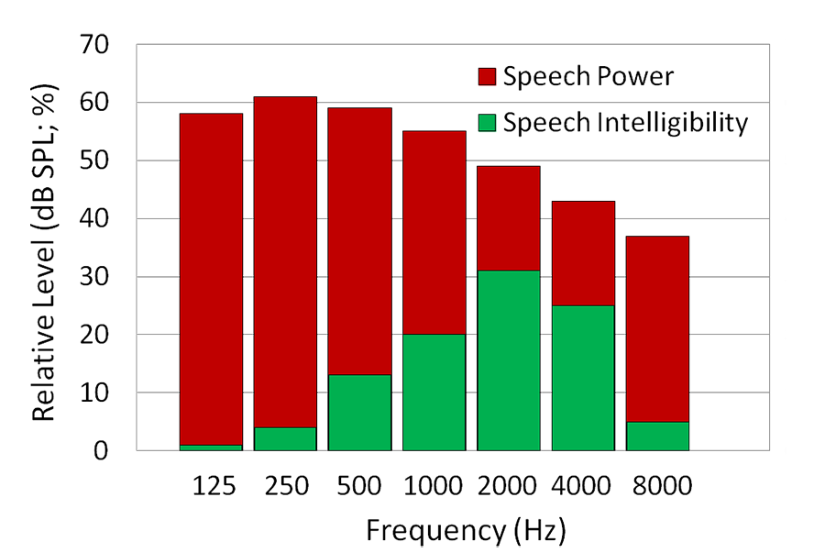
\includegraphics[width=1\textwidth]{speech_intelligibility}
		\caption{The figure shows the power and intelligibility in octave  \citep{arl_us_army}}
		\label{fig:speech_intelligibility}
\end{figure}

As it can be seen in \autoref{fig:speech_intelligibility}, the frequency range can be further limited between \SI{355}{\hertz} and \SI{5.68}{\kilo\hertz} because of the outer low frequency limit of the \SI{500}{\hertz} octave band and the upper outer high frequency limit for the \SI{4}{\kilo\hertz} octave band. 

This is also supported by the inequal distribution of vowels and consonants in words in terms of speech intelligibility. As explained in \citep{arl_us_army}, consonants are the dominant part, and the reason can be found in the relation between speech power and intelligibility(\autoref{fig:speech_intelligibility}), as vowels (which have higher power) fall into the low frequency region, while consonants (lower power) are located in a higher frequency range.

\subsection{Conclusion}
Taking all of the previously stated points into account, it can be concluded that for a transducer to be effective in speech transmission, it must, at least, have a good frequency response in the frequency range from \SI{355}{\hertz} up to \SI{5.68}{\kilo\hertz} to establish a good speech intelligibility in a communication system.

